\documentclass[letterpaper]{article}
% \usepackage{usenix2019_v3}

% to be able to draw some self-contained figs
\usepackage{tikz}
\usetikzlibrary{shapes.geometric}
\usetikzlibrary{positioning}
\usepackage{amsmath}
\usepackage{url}
\usepackage{algpseudocode}
\usepackage{algorithm}
\usepackage{graphicx}
\usepackage{setspace}
\usepackage{svg}
\graphicspath{ {./diagrams/} }
\doublespacing

% inlined bib file
% \usepackage{filecontents}

\AtBeginDocument{%
  \providecommand\BibTeX{{%
    Bib\TeX}}}

%-------------------------------------------------------------------------------
\begin{document}
%-------------------------------------------------------------------------------

%don't want date printed
\date{}

% make title bold and 14 pt font (Latex default is non-bold, 16 pt)
\title{3Tree: Segmented CPU Caching for Speed and Eviction Set
  Security}

%for single author (just remove % characters)
\author{
{\rm Rishav Chakravarty}\\
Dartmouth College
% copy the following lines to add more authors
% \and
% {\rm Name}\\
%Name Institution
} % end author

\maketitle

%-------------------------------------------------------------------------------
\begin{abstract}
%-------------------------------------------------------------------------------

  Eviction sets are fundamental to cache-enabled attacks such as Rowhammer
  and Prime+Probe style side channel attacks.
  Previous work focuses on defending against finding eviction sets for one or many
  of a cache's sets ("mapping" the cache).

  In this paper we present the replacement policy of a CPU cache as a defense against
  % Possibly: add mapping as a defense target too
  the use of already-found eviction sets to occupy cache sets ("priming" the cache),
	and against the use of eviction sets to induce targeted electrical interference in DRAM cells.
  In particular, we establish a relation between the cache replacement policy and the
  maximum data leakage throughput of a Prime+Probe style attack as well as the
  maximum DRAM access in Rowhammer style attacks.

	Finally, we present three novel CPU cache replacement algorithms:
	SIEVE, based on the software SIEVE algorithm,
	2Tree, based on the TwoQ and SLRU software algorithms,
	and 3Tree, an enhancement of 2Tree.
	Many variants of 2Tree and 3Tree are presented and tested, including
	set dueling used to switch between two variants of 3Tree.
  A CPU implementation of SLRU (along with many performance-enhancing variations) has
  already been introduced, and 3Tree and SIEVE are competitive in performance.
  In gem5 PARSEC simulations, 3Tree incurs a 1.7 percentage point miss ratio penalty
  compared to TreePLRU and SIEVE incurs a 2.2 percentage point penalty.
  Most importantly, 3Tree and SIEVE significantly enhance the security against eviction set
  cache priming.
  3Tree shows a median 94.6\% reduction in the data leakage throughput through Prime+Probe attacks,
  and SIEVE shows a median 92.7\% reduction.

\end{abstract}

%-------------------------------------------------------------------------------
\section{Introduction}
%-------------------------------------------------------------------------------

CPU caches are increasingly becoming vectors and targets for modern attacks.
The most common are software attacks that take advantage of the architecture.
Prime+Probe attacks use the sharing of a cache among multiple processes and sometimes different cores
to leak information from a different address space,
even though processes have their memory isolated from one another.
This includes attacks that use this form as their foundation,
such as speculative execution attacks
\cite{Gofetch}
\cite{Spectre}
\cite{Meltdown}
\cite{TikTag}
\cite{PACMan}
\cite{SPAM}
\cite{LeakyWay}
\cite{Streamline}
\cite{TransientAttackSurvey}.
Rowhammer attacks use the cache to attack the DRAM modules
by repeatedly touching a memory address until the electrical interference induces a targeted bitflip
\cite{Rowhammer}.
Attacks like these are able to leak significant amounts of information from victim processes.
% How much can Spectre leak? Rowhammer? Gofetch?
Additionally, many of these attacks are difficult to detect and prevent as they occur.
Speculative attacks are especially silent,
as they work within the window of transient execution,
which completely deletes any easily accessible trace of execution after it is flushed.

Many software approaches have been introduced to defend against these attacks,
including Rowhammer-specific defenses
\cite{RowhammerDefense} % TODO: cite one more
and many defenses against Spectre and Meltdown at the OS level that are currently in use
% TODO: cite some Spectre OS defense
.

Hardware defenses are less common because changing the cache architecture can have
significant performance implications,
and preventing eviction set-based attacks completely can severely degrade
cache capacity and performance.
Instead, hardware defenses usually focus on slowing these attacks
by introducing complexity in eviction set-specific function
without overly affecting normal performance.
While software defenses benefit from being dynamic
and can be patched into operating systems and maintained applications,
many applications are archaic or unmaintained, and different hardware may secure these systems
where software alone cannot.

Both Rowhammer and Prime+Probe-based attacks use \textit{Eviction Sets}
as the foundation of their attack.
Many procedures have been introduced to very quickly discover these eviction sets,
whether for a single cache set \cite{TPFES}
or for a majority of the cache \cite{EvictionSetsAtScale}.
However, these algorithms make assumptions about the architecture,
including the use of LRU or Random replacement algorithms
and, critically, the lack of modern CPU features like skewed caches
% TODO: get examples of cache randomization from Prune+PlumTree
\cite{EvictionSetsAtScale}.
Additionally, these algorithms enable or enhance the setup for cache attacks,
but do not address the execution of the attack itself.

To this end, we introduce the \textit{SIEVE}, \textit{2Tree}, and \textit{3Tree} cache replacement algorithms.
The algorithms are based on software cache eviction algorithms that focus on
performance enhancement over other very commonly used algorithms,
and we implement variation of the algorithms in hardware
with these performance characteristics in mind
and with an emphasis on security against cache priming.

\section{Background}
% Introduce the concepts of caches and eviction sets

Caches are memory modules between processors and larger, slower memory modules.
They are used in many computing environments where the latency of memory
is a significant factor in performance,
such as small databases between clients and CDNs; we observe caches in CPUs.

In order to take advantage of the spatial and temporal locality characteristics
of most computing workloads,
CPU memory caches are divided into \textit{cache lines}, usually 64 bytes long,
grouped into \textit{sets} usually of 1-16 lines.
The number of lines per set is called the associativity, which we hence call $a$.
Modern CPUs use multiple levels of caches, including an L1, L2, and optional L3 cache
in order of increasing size and distance from the CPU.
The Last Level Cache (LLC) is often shared among all CPU cores, and may further group
cache sets into \textit{slices}, with one or two slices placed physically on each core.
Smaller caches tend to have lower associativity values of 2 or 4, and larger caches and LLCs
tend to have higher values between 4 and 16.

As caches are limited in size, replacement policies, also called eviction algorithms,
replace an old or stale cache line (an \textit{eviction candidate}) with a new one,
chosen based on per-object metadata.
The ideal replacement algorithm minimizes \textit{cache misses}, where the requested memory address
is not present in the cache and must wait much longer for a response
from a larger cache or main memory.
An efficient replacement algorithm will evict objects that are predicted to be unused
or will induce \textit{thrashing}, where sequential memory touches are all cache misses,
and conversely will retain objects that are commonly used
or predicted to be used again in the near future.
The miss ratio describes the efficiency of a cache:
\begin{equation}
  m = \frac{misses}{hits + misses}
\end{equation}
A cache may also be measured by its latency $T$, which describes the amount of time taken
to fulfill a memory request.
Together, the memory access time performance of a cache is given by the equation:
\begin{equation}
  T = T_{L1}(1-m_{L1}) + T_{L2}m_{L1}(1-m_{L2}) + \dots
\end{equation}

\subsection{Pseudo LRU}
% DIAGRAM: Bit Tree
% Explain how it works
% Explain what's good about it and why it's so often used
% Describe QLRU in Intel caches, why it's used, etc.

Tree Pseudo Least Recently Used (TreePLRU) is a very common replacement algorithm that
very closely follows the function of LRU.
As a perfect LRU hardware implementation requires a complex circuit and lots of energy usage,
this approximation is commonly used to approach the performance of LRU.
It organizes the cache lines into a binary tree structure to recursively divide the cache
into "hot" and a "cold" subtrees.
Each node in the tree is a single bit that 'points' to one half of the tree
(e.g. 0 points to the left, 1 points to the right).
Eviction candidates are chosen by tracing down the tree according to the direction of these nodes
following each node's colder subtree,
and address touches (including the initial placement into the cache)
trace from the node up the tree and set each node to point away from the cache line,
as the cache line should in all levels be in the "hot" subtree.
This algorithm can be easily extended into First In First Out (FIFO)
by only placing objects into the Most Recently Used (MRU) position when they are first added
and not updating the tree upon subsequent address touches.

%----------------
% TreePLRU Diagram
%----------------
\begin{figure*}
\begin{center}
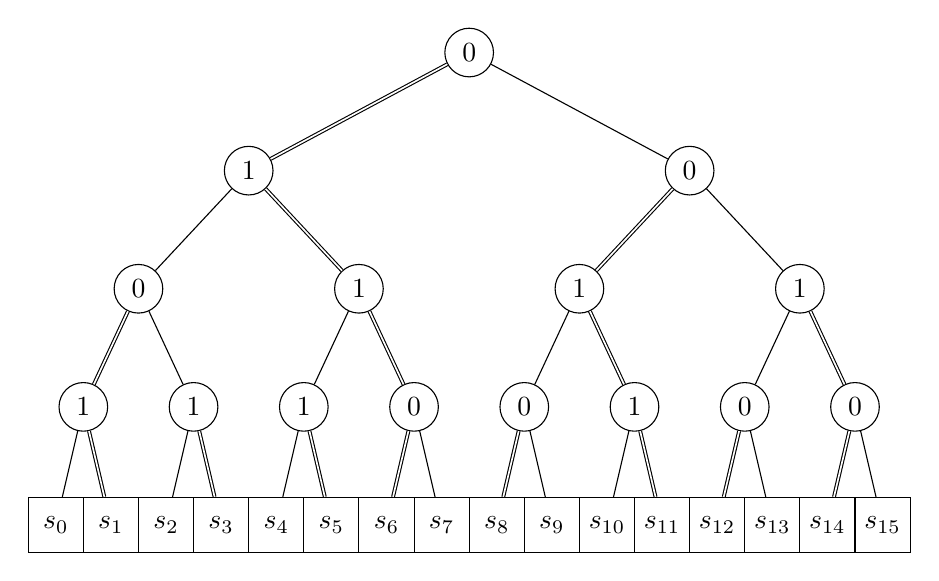
\begin{tikzpicture} [
  every node/.style={draw,distance=12mm},
  level 0/.style={circle},
  level 1/.style={circle,sibling distance=56mm},
  level 2/.style={circle,sibling distance=28mm},
  level 3/.style={circle,sibling distance=14mm},
  level 4/.style={rectangle,minimum size=7mm,inner sep=0,sibling distance=7mm}
  ]
  \node (n0) [circle] {0}
    child {
      node (n1) {1}
      child {
        node (n3) {0}
        child {
          node (n7) {1}
          child {
            node (n15) {$s_0$}
          }
          child {
            node (n16) {$s_1$}
          edge from parent [double]}
        edge from parent [double]}
        child {
          node (n8) {1}
          child {
            node (n17) {$s_2$}
          }
          child {
            node (n18) {$s_3$}
          edge from parent [double]}
        }
      }
      child {
        node (n4) {1}
        child {
          node (n9) {1}
          child {
            node (n19) {$s_4$}
          }
          child {
            node (n20) {$s_5$}
          edge from parent [double]}
        }
        child {
          node (n10) {0}
          child {
            node (n21) {$s_6$}
          edge from parent [double]}
          child {
            node (n22) {$s_7$}
          }
        edge from parent [double]}
      edge from parent [double]}
    edge from parent [double]}
    child {
      node (n2) {0}
      child {
        node (n5) {1}
        child {
          node (n11) {0}
          child {
            node (n23) {$s_8$}
          edge from parent [double]}
          child {
            node (n24) {$s_9$}
          }
        }
        child {
          node (n12) {1}
          child {
            node (n25) {$s_{10}$}
          }
          child {
            node (n26) {$s_{11}$}
          edge from parent [double]}
        edge from parent [double]}
      edge from parent [double]}
      child {
        node (n6) {1}
        child {
          node (n13) {0}
          child {
            node (n27) {$s_{12}$}
          edge from parent [double]}
          child {
            node (n28) {$s_{13}$}
          }
        }
        child {
          node (n14) {0}
          child {
            node (n29) {$s_{14}$}
          edge from parent [double]}
          child {
            node (n30) {$s_{15}$}
          }
        edge from parent [double]}
      }
    };
\end{tikzpicture}
\end{center}
  \caption{
		TreePLRU metadata structure. In this cache state, $s_6$ will be the first cache object evicted,
		followed by $s_{11}$. $s_{13}$ is in the MRU position and the farthest from eviction.
	}
  \label{fig:treeplru}
\end{figure*}

Quad Least Recently Used (QLRU) is another replacement algorithm
commonly used in Intel processors and used to replicate the function of LRU.
It is very similar to RRIP \cite{RRIP}, using four possible priority values for each cache line.
New objects are added with a low priority which gets promoted upon touches of the same address.
The object with the lowest priority is evicted, using the order of the cache lines to break ties.

\subsection{Random Replacement}
% Explain how it works
% Explain what's good about it and where it's conditionally used

Random Replacement is an eviction algorithm sometimes used in CPU caches.
Upon a cache miss, this algorithm simply chooses an eviction candidate at random.
As this algorithm does not attempt to evaluate cache lines for recency of use
or predict their next use, it suffers from a higher miss ratio than many other algorithms.
However, since it requires no cache metadata and no algorithm logic,
it uses very little energy and incurs no extra latency.
For this reason, Random Replacement is sometimes used in L1 caches.
The low latency of these caches, which is usually around 1-2 nanoseconds for L1
and 4-5 nanoseconds for L2 to fulfill a memory request,
means that the more common cache misses do not add too much latency to memory requests
but may save a lot of energy.
Most ARM processors equip Random Replacement algorithms in some of their CPU caches.
% TODO: cite

\subsection{TwoQ and SLRU}
% Explain how it works
% Explain what's good about it and where it's used (not hardware)

TwoQ \cite{TwoQ} and Segmented Least Recently Used (SLRU) \cite{SLRU}
are very similar eviction algorithms implemented in software,
enhancing miss ratio performance in caches for large web caches and CDNs
and for smaller-scale caches like those used in Disk-IO interaction.
They both split the LRU queue into two segments, one holding older, warmer objects
which we hence call the "hot" queue,
and one holding colder or younger objects,
which we call the "cold" queue.

Both algorithms add new objects to the cold queue
and then promote them to the head of the hot queue upon a subsequent touch.
Upon promotion, one object must be removed from the hot queue;
SLRU solves this by choosing the object in the LRU position as an eviction candidate
and placing it at the Most Recently Updated (MRU) position in the cold queue,
and TwoQ solves this by removing the object from the cache altogether.
This way, cold queue objects are isolated from the hot queue unless they are touched again,
preventing against cache thrashing and making the cache scan-resistant.

Later variations of SLRU have been introduced \cite{SSLRU},
including hardware implementations for CPU caches
\cite{DuelingSLRU}\cite{LimitedSLRU}\cite{FixedSLRU}\cite{FixedSLRUEnhancements}.
These algorithms perform well but introduce significant overhead in hardware complexity,
using bypass tables.

\subsection{SIEVE}

SIEVE is a simple algorithm used for large software caches as both an eviction algorithm
and as a cache primitive used as a foundation for other, more complicated algorithms. \cite{SIEVE}
It improves upon LRU and FIFO Reinsertion,
in which elements are placed in a FIFO queue with a \textit{safe} boolean:
upon a touch, the element is marked as safe, and upon eviction,
the first non-safe object is evicted.

SIEVE uses only one boolean of metadata per cache line, \textit{visited}
as well as a \textit{hand} to trace through the cache.
When touched, cache objects are marked as visited.
Upon eviction, the hand marches through the cache array, returning to the head if at the tail;
it evicts the first element that has its \textit{visited} bit unset,
and unsets the \textit{visited} bits of any cache objects it traces through along the way.
Instead of placing the new object at the eviction position,
the algorithm always places new objects at the head of the queue,
which prevents the new and the retained objects from being mixed together.
The hand persists its position between cache operations,
effectively resulting in a sliding window of objects at risk of eviction.

This algorithm shows significant average improvements in CDN workflow miss ratio
over many eviction algorithms,
including LRU, FIFO, ARC, and TwoQ, while being simpler than these alternatives.
It is based on principles of \textit{lazy promotion},
in which objects are only promoted at eviction time,
and \textit{quick demotion}, in which most new objects are removed quickly after their insertion.
Additionally, it significantly improves over the data usage of other
software caching algorithms, as the single boolean of metadata per line and the hand
are small and constant in memory size regardless of the capacity of the cache,
whereas timestamps for algorithms like LRU must each contain much more data,
and other index-based ordering schemes must increase their memory footprint for increasing cache size.
The algorithm also has an advantage in multithreaded software caches;
since only the visited bit of an object is set upon a cache object touch,
only cache evictions require a lock on the whole cache array.
For multithreaded applications, this vastly improves throughput,
as most other contemporary cache eviction algorithms require a whole-cache lock
both evictions and touches.

\subsection{Eviction Sets in Attacks}
% Both of the above attacks use eviction sets
% Define an eviction set very thoroughly
% Discovery and Occupation
% Actually sike covert channels can optionally use other forms
% but this is the universal way of doing it (not just Intel)
% How is it used in these attacks?

Eviction sets are an attack primitive used in many cache-based hardware attacks,
including Prime+Probe and Rowhammer.
They are used to \textit{prime} a cache by ensuring that a victim object is removed from its cache set.
An eviction set is a group of virtual addresses that are all congruent: they all map to the same cache set.
For an $a$-way associative cache, an eviction set $S$ must contain $|S| \geq a$ addresses.

The first step in eviction set-based attacks is \textit{discovery},
where an attacker must reduce a set of randmly chosen memory addresses
into a \textit{minimal eviction set}, where $|S| = a$.
Algorithms have been outlined to efficiently find eviction sets for one or almost all
of the cache sets.
% TODO: is there much else I need to write for this?

% Timing oracle
Eviction sets are used in Prime+Probe attacks as a timing oracle.
After finding eviction sets and using them to prime the cache,
an attacker times access to all items in the target cache set
before and after a victim program is run and possibly accesses elements in these target sets.
A greater time after the victim program implies that the victim accessed addresses in the victim set,
replacing eviction set elements which, upon the second access,
must introduce the significantly longer latency of a DRAM access.

Eviction sets are used in Rowhammer to bypass the cache and force DRAM hits.
By priming a cache set to evict a target congruent target address from all levels of the cache,
the target address will have to access the RAM.
Due to % TODO: what is this called
repeated RAM hits can encourage bitflips in victim memory.

\subsection{Cache-enabled Attacks}
Caches are mostly well-protected against direct attacks;
users are prevented from accessing memory placed in the cache by another process.
However, the cache can serve as a tool to enable other attacks,
especially as a side channel with a timing oracle to leak information.

\subsubsection{Transient Attacks and Forms}
Transient attacks, also called speculative execution attacks, take advantage of modern CPUs' speculative execution pipeline.
Speculative execution increases performance by guessing uncertain values that take time to evaluate, such as branch destinations
and conditions, and continuing execution under the assumption of the guess;
if the guess is later found to be incorrect, the CPU flushes the pipeline and rolls back to the last checkpoint known to be correct.

The speculative window - the period between a condition starting speculative execution and its value confirmation -
introduces a vulnerability;
If the guessed condition was incorrect, malicious code may be run in the speculative window.
Many modern CPUs, prioritizing performance, roll back only as much data as is required to continue execution
with correct functionality; code in the speculative window can leave traces in a covert channel in hardware
components where speculative misses are not rolled back.

As outlined by Xiong, et. al \cite{TransientAttackSurvey}, transient execution attacks take advantage of this speculative execution window in three steps:
\begin{enumerate}
    \item \textit{Setup Phase}:
An attacker primes the microarchitectural state such that victim actions can later be decoded and intrepreted
    \item \textit{Transient Execution Phase}:
Speculative execution takes place, usually induced in a victim process by the attacker using a disclosure gadget.
The malicious code runs in the speculative window, quietly leaving a trace in the primed covert channel.
This attacking code is then squashed by the speculative execution pipeline, but the trace remains.
    \item \textit{Decoding Phase}:
An attacker decodes the information leaked into the covert channel during the Transient Execution Phase.
\end{enumerate}

As the CPU cache is too large to fully roll back upon a speculative miss, this is a common side of transient information leakage.
Previous hardware solutions to transient attacks include MuonTrap \cite{MuonTrap},
which introduces an additional L0-level cache that catches all speculative memory accesses
and can easily roll back upon a speculative miss.

Spectre and Meltdown, with victim-executed speculative execution and exception-induced speculative execution respectively, 
are early examples of transient attacks.
New transient attacks like PACMAN, TikTag, GoFetch, and more, use other components and features of the CPU.
These attacks follow many different forms depending on the capabilities of the hardware they run on and the
nature of the process they seek to attack.
We focus on defending against the following forms:
\begin{enumerate}
    \item \textit{Prime+Probe}:
An attacker primes a known location in cache, executes a victim program, and determines 
if the victim program accessed the primed location. This is a very common and relatively simple
type of transient execution attack.
    \item \textit{Evict+Reload}:
An attacker loads a shared binary object into its address space and primes the cache for an address
in the shared binary.
After executing the victim program, the attacker determines if the victim program accessed the primed location.
    \item \textit{Evict+Time}:
An attacker first measures the execution time of a victim program.
After priming the cache, the victim process is run and timed again.
A timing difference implies that the victim process accessed the memory affected by the cache priming.
\end{enumerate}

These attack forms are applicable to transient attacks and many others to establish a covert channel in the cache for information leakage,
and they all use eviction sets to prime the cache.
We aim to prevent or slow the use of eviction sets in the \textit{setup phase} of the transient attack, which will decrease the throughput of information leakage.

\subsubsection{Rowhammer}

Rowhammer takes advantage of electromagnetic coupling
between increasingly small and densely compacted DRAM cells.
DRAM consists of memory cells, and modern chip design techniques attempt to compact these cells
very close together to maximize energy efficiency and memory capacity.
The extreme proximity of these cells and the necessity of charge refreshing
due to the lack of charge persistence means many accesses to a memory address
in quick succession can spontaneously induce charge interference \em a bit flip \em
in adjacent memory rows in a cell bank.
Rowhammer attacks use repeated targeted memory accesses to induce bitflips in specific memory locations,
and may result in consequences like incorrect privilege elevation.

Notably, this attack requires a method of bypassing the cache.
As write-back caches store all memory requests and prevent DRAM access for addresses contained in the cache,
directly repeated accesses to a single target address would simply touch the cache
and have no effect on the RAM cells.
In systems that have the \texttt{clflush} instruction enabled,
attackers may flush the cache after each access,
thus requiring the memory request to fetch from DRAM.
In systems where this instruction is disabled or does not exist,
attacks often use eviction sets to force DRAM access.


\subsection{Eviction Sets}
Eviction sets are an attack primitive used in many cache-based hardware attacks.
They are used to prime a cache by ensuring that a target object is removed from its cache set.
An eviction set is a group of virtual addresses that are all congruent: they all map to the same cache set.
For a cache set with associativity $a$, an eviction set $S$ must contain $|S| \geq a$ addresses.
In a system that does not use pseudo-random mapping from physical addresses to cache sets,
congruent addresses share index bits in their corresponding physical address.

% An attacker may use an eviction set to fill a target cache set with attacker-provided objects; we refer to this process as \textit{occupation} of an eviction set.

Eviction sets are used in the following steps:

\begin{enumerate}
    \item \textit{Creation:} An attacker finds a set of congruent virtual addresses $S$ for $a$-associativity cache with $|S| \geq a$. Optionally, the attacker may choose a minimal eviction set with $|S|=a$.
    Although minimizing the eviction set can simplify the accurate detection of information leakage,
    many attacks are successful with eviction sets larger than their target caches.

    \item \textit{Occupation:} An attacker touches the memory addresses in the eviction set until the target cache is entirely filled with memory addresses from the eviction set.
    Anything previously in the cache set should be evicted through this process.
    This step is often called \textit{priming the cache} – we refer to this process as cache set \textit{occupation}.
\end{enumerate}

In rowhammer attacks, eviction sets are used to ensure that an attacker's memory request reaches DRAM.
The attacker repeatedly touches a target address, evicts the target address so subsequent accesses will not be caught by the cache,
and re-references the target address.

In transient attacks, a target address is usually evicted as part of a timing attack, as a memory request to an evicted object
must take time to travel to and from DRAM, and this timing difference is significant enough to be measured
by high-performance counters or simply by a continuously incrementing variable.
In Prime+Probe, the attacker occupies the cache set of a target address, executes the victim program, and re-references
all the addresses in the eviction set; an increase in the time taken implies that the target address was referenced and evicted
one of the objects of the eviction set.
In Evict+Reload and Evict+Time, the attacker measures the victim's runtime before and after occupying a cache set,
with a longer re-run time implying a reference of an evicted cache object.

We primarily aim to slow cache set \textit{occupation}.
Most eviction set attacks create eviction sets once but use them for occupation many times;
by slowing occupation, we reduce the information leakage throughput of these attacks
and possibly reduce the likelihood of rowhammer bitflips.

\section{Design}

We seek to make rowhammer-style and transient execution attacks more difficult by preventing or slowing the use of eviction sets
using hardware-level cache eviction algorithms.
Additionally, we aim to accomplish this security without inducing a significant performance hit in the cache of either miss rate or latency.

\subsection{Expected Difficulty of an Eviction Algorithm}
We define the difficulty $D$ of occupying a cache set with a certain touching pattern
as the total number of memory touches required to overwrite all lines in the cache
with addresses from an eviction set.

For the minimum difficulty $D_m$, we assume an optimal attacker;
for each eviction algorithm, there exists a memory touching pattern that
most effectively primes a cache set.
In this case, an optimal attacker does not know the state of the cache,
but may optionally use a timing oracle to determine if a previously touched address
is still in the cache.
This timing oracle incurs an extra counted touch, but we ignore the cost of
the added conditional.

Additionally, randomness is a factor in some of these eviction algorithms.
We assume a uniform random distribution of initial cache states;
We define the expected minimum difficulty $D_{Em}$ of an eviction algorithm
as the mean number of optimally-ordered touches required to fill a cache set.

Finally, SLRU and our implementation of 3Tree splits the cache into segments,
which may mean that the attacker can guarantee that a victim overwrites
an attacker-primed address without the attacker filling the entire cache set,
and thus that the minimum expected difficulty may be higher than the true value
when used in an attack.
We define the guarantee difficulty $D_g$ as the minimum expected number of touches
required to guarantee an attacker access to an accurate timing oracle.
For replacement algorithms where new objects may be placed in any index in the cache,
$D_g = D_{Em}$, as an attacker must fill every cache line to guarantee
that a victim touch will overwrite an eviction set address.
We separately define $D_g$ for 2Tree.

\subsubsection{LRU, TreePLRU, and FIFO}
% Derive expected difficulty, no choice or permutation randomness
LRU, TreePLRU, and FIFO pose little defense against cache priming.
In both FIFO and LRU caches, new cache objects are instantly promoted to the head of the queue.
In LRU, new objects are marked as the most recently updated and thus the last to be evicted,
and the FIFO queue means new objects are evicted after objects added earlier.
Although TreePLRU does not follow the same linear structure,
it is similarly trivial to occupy a cache set.
Thus, for an $a$-way associativity LRU, FIFO, or TreePLRU cache, an attacker only needs
$a$ sequential touches to fill a cache set.
As these algorithms are deterministic, the expected difficulty is the same value.

\begin{equation}\label{LRUExpectedD}
  D_g(\text{LRU}) = D_m(\text{LRU}) = D_{Em}(\text{LRU}) = a
\end{equation}

\subsubsection{Random Replacement}
Given a cache set with associativity $a$ in which an attacker has occupied $n$ addresses
using some subset $S \subset E, |S| = n$ of eviction set $E$,
a following touch on address $\alpha$ may be in $S$ or not.

If $\alpha \in S$, there is no cache or per-line metadata to update, and the cache state does not change.

If $\alpha \notin S$, the random replacement algorithm will evict an address $\beta$.
This evicted address will occupy an unoccupied line with probability
$P(\beta \notin S) = \frac{a-n}{a}$.

Then, the probability occupying $n+1$ addresses in a cache set with $n$ addresses occupied is $P(n+1) = \frac{a-n}{a}$.
The corresponding expected value is $EV(n+1) = \frac{1}{P(n+1)} = \frac{a}{a-n}$
Then, the expected value of the total number of unique touches to occupy an eviction set is

% If they have an issue with this not being fully simplified they can take that up in review
\begin{equation}\label{RandomExpected}
    D_g(\text{Random}) = D_{Em}(\text{Random}) = \sum_{i=0}^{a-1}{\frac{a}{a-i}}
\end{equation}

\subsection{Preventing Eviction Set Occupation}
Attackers use eviction sets as attack primitives to guarantee that a target address is not present in the cache
so a victim's memory request of the target address must travel to DRAM and back.
Leaving at least one of the lines in a cache set open and unoccupied means that attackers have no guarantee that the target address is evicted.
Thus, to slow the use of an eviction set in occupying a cache set, we must only increase the difficulty of the eviction algorithm used.

\subsection{Latency and Energy Costs}

As the CPU implements eviction algorithms in hardware, the function of some software-based algorithms
may not be exactly reflected without inducing significant performance or complexity overhead.
For example, LRU can be implemented in a software cache to add, update, and remove objects in $O(1)$ time.
Although no such time complexity exists for algorithm circuitry that runs in parallel,
exact LRU is complex in CPU caches and involves lots of metadata per cache line and lots of circuitry to
determine an eviction candidate.
Excessive circuitry introduces extra latency by increasing the critical path of the circuit
and extra energy usage by requiring additional transistors.
The LRU algorithm is thus commonly simplified to TreePLRU in the CPU, which requires much less hardware complexity
but achieves a similar miss ratio.
Although the energy usage can be significant, modern CPU features like prefetching largely mitigate the latency factor of the algorithm.
Additionally, many modern CPUs punt the cache eviction calculation to after fulfilling the memory request.

Additionally, the cache - other than random replacement caches - may introduce registers for the cache metadata used in eviction.
However, the amount of metadata is much smaller than the amount of data in a cache set:
for an 8-way associative, 64-byte cache line, a TreePLRU replacement policy for the set uses
$\frac{7}{512 \cdot 8}=0.17\%$ as much space as the data itself.
Thus, within reason, we treat metadata usage as insignificant compared to the space and energy usage of the cache.

For the sake of simplicity and due to the lack of comparison against proprietary CPU cache implementations,
we analyze and evaluate our eviction algorithm qualitatively.
% I mean to say that we only check that the value is reasonable and move on,
% because that's all I can do

\subsection{Miss Rate Cost}

Finally, we try to optimize our algorithms for cache miss rate.
Miss ratios in the CPU are usually quite low,
given the high spatial and temporal locality of memory accesses
and the need for extreme speed in these caches.
We use TreePLRU as a baseline for performance,
as it is likely the most commonly used CPU replacement algorithm
and performs reasonably well in most workloads.

\section{Implementation}

As discussed in 3.3, due to the hardware requirements and parallel nature of circuits,
we implement our cache eviction algorithms as approximations of their software equivalents.
We implement and discuss multiple variants of each algorithm.

\subsection{SIEVE}

SIEVE, as implemented in software, does not translate well to hardware.
It relies on entirely sequential logic to determine an eviction candidate;
additionally, it conditionally returns the hand to the beginning of the cache array.
These two features imply the use of a register to keep track of the hand position,
constant updating to reflect its marching through the cache array
and its possibility of returning to the beginning of the array.
Along with an increased hardware footprint, this would result in immense energy usage,
especially compared to other algorithms like TreePLRU that select an eviction candidate
without sequential logic at all.

\begin{figure*}
	\begin{center}
		% \includesvg{diagrams/Sieve.svg}
	\end{center}
	\caption{SIEVE metadata structure}
	\label{fig:sieve}
\end{figure*}


We implement SIEVE in the cache by dividing the cache objects into four groups with two boolean tags.
First, we use a \textit{safe} bit analogous to the position of the cursor in software SIEVE.
In the software version, objects to the right of the cursor are the closest to being checked for the visited bit,
and objects to the left of the cursor are relatively safe from being checked.
We represent an object to the left of the cursor with an enabled safe bit
and objects to the right of the cursor with a disabled safe bit.
Then, we use a \textit{visited} bit very similar to the software implementation of SIEVE,
which is set to 1 when a cache object is added or touched.
The algorithm first makes checks to ensure that there will be a valid eviction candidate.
It determines if all of the objects are safe,
and in this case disables all of the safe bits.
This is analogous to the cursor in software SIEVE traversing the whole cache and looping back to the beginning of the array.
It also checks if all of the objects are visited,
and in this case disables all of the visited bits.
This is analogous to the cursor traversing an entirely visited array and looping back to its start position,
resetting all of the \textit{visited} booleans along the way,
before continuing on.
Checking these boundaries is possible in hardware and prevents the algorithm from
searching for an eviction candidate while changing values
and having to make a second pass to find a valid eviction candidate based on the changed values.
Then, the algorithm marches through the cache lines in the order of their position in the cache
and checks each element.
The first cache object that is not marked \textit{visited} is evicted,
and the lines before it are all marked as unsafe.

Unlike a raw implementation of SIEVE, this algorithm can be implemented using a Priority Encoder
to search along the cache lines without requiring registers or extra clock cycles.

\subsection{2Tree}

TwoQ does not rely on sequential logic nearly as much as SIEVE,
but there are multiple possible ways to implement the dual-queue structure.
I implement TwoQ as a tree structure very similar to TreePLRU, as shown in figure \ref{fig:2tree}.
The cache is split into two smaller queues, each with their own subtree:
the \textit{cold} queue, containing $\frac{1}{4}$ of the elements,
and the \textit{hot} queue, containing $\frac{3}{4}$ of the elements.
The hot queue, having a multiple of 3 elements,
is further marked with
a \textit{probation} segment, containing $\frac{1}{4}$ of the total elements,
and a \textit{safe} segment, containing the remaining $\frac{1}{2}$ of the elements.
We choose a tree-based replacement policy for each of the two subtrees,
and additionally define a \textit{choice} probability $c$.

With this structure, the cold tree,
not including the cache lines themselves as leaf nodes, has height $log(a) - 2$.
Thus, this algorithm is not possible for caches with $a < 4$.
We implement and test this algorithm only for 4-, 8-, and 16-way associativity.

New elements are added to the cold queue with probability $1 - c$
or to the probation segment of the hot queue with probability $c$.
If added to the cold queue, an eviction candidate is selected from the cold queue
according to the cold queue's replacement algorithm;
if added to the probation queue, the eviction candidate is selected using the replacement algorithm
of the hot queue, but limited to the subtree of the probation queue.
When an object $a$ in the cold queue is touched again
or a new object is added directly to the probation queue,
an eviction candidate $b$ is chosen from the hot queue according to its replacement algorithm.
The entire cache line of $a$ is swapped with that of $b$,
and $a$, now in the hot queue, is promoted according to the hot queue's replacement policy.
$b$, now in the cold queue, is not promoted.

%----------------
% 2Tree Diagram
%----------------
\begin{figure*}
\begin{center}
\begin{tikzpicture} [
  every node/.style={draw,distance=12mm},
  level 0/.style={circle},
  level 1/.style={circle,sibling distance=56mm},
  level 2/.style={circle,sibling distance=28mm},
  level 3/.style={circle,sibling distance=14mm},
  level 4/.style={rectangle,minimum size=7mm,inner sep=0,sibling distance=7mm}
  ]
  \node (n0) [circle, label=above:Hot] {0}
		child [circle, sibling distance=28mm] {
			node [
				left=22mm of n5,
				label=left:Probation
			] (n4) {1}
				child [circle,sibling distance=14mm] {
          node (n9) {1}
					child [rectangle,minimum size=7mm,inner sep=0,sibling distance=7mm] {
            node (n19) {$s_4$}
          }
					child [rectangle,minimum size=7mm,inner sep=0,sibling distance=7mm]{
            node (n20) {$s_5$}
          edge from parent [double]}
        }
				child [circle,sibling distance=14mm] {
          node (n10) {0}
					child [rectangle,minimum size=7mm,inner sep=0,sibling distance=7mm]{
            node (n21) {$s_6$}
          edge from parent [double]}
					child [rectangle,minimum size=7mm,inner sep=0,sibling distance=7mm]{
            node (n22) {$s_7$}
          }
        edge from parent [double]}
      edge from parent [double]}
    child {
			node [label=above:Safe] (n2) {0}
      child {
        node (n5) {1}
        child {
          node (n11) {0}
          child {
            node (n23) {$s_8$}
          edge from parent [double]}
          child {
            node (n24) {$s_9$}
          }
        }
        child {
          node (n12) {1}
          child {
            node (n25) {$s_{10}$}
          }
          child {
            node (n26) {$s_{11}$}
          edge from parent [double]}
        edge from parent [double]}
      edge from parent [double]}
      child {
        node (n6) {1}
        child {
          node (n13) {0}
          child {
            node (n27) {$s_{12}$}
          edge from parent [double]}
          child {
            node (n28) {$s_{13}$}
          }
        }
        child {
          node (n14) {0}
          child {
            node (n29) {$s_{14}$}
          edge from parent [double]}
          child {
            node (n30) {$s_{15}$}
          }
        edge from parent [double]}
      }
    };
	\node [left=22mm of n4, circle, label=above:Cold](n3) {0}
		child [circle, sibling distance=14mm] {
				node (n7) {1}
				child [rectangle,minimum size=7mm,inner sep=0,sibling distance=7mm] {
					node (n15) {$s_0$}
				}
				child [rectangle,minimum size=7mm,inner sep=0,sibling distance=7mm] {
					node (n16) {$s_1$}
				edge from parent [double]}
			edge from parent [double]}
			child [circle, sibling distance=14mm]{
			node (n8) {1}
			child [rectangle,minimum size=7mm,inner sep=0,sibling distance=7mm]{
				node (n17) {$s_2$}
			}
			child [rectangle,minimum size=7mm,inner sep=0,sibling distance=7mm]{
				node (n18) {$s_3$}
			edge from parent [double]}
		};
\end{tikzpicture}
\end{center}
  \caption{
		2Tree metadata structure, with Cold, Probation, and Hot subtrees.
		If the cold subtree is chosen for eviction with probability $c$,
		$s_1$ will be the evicted.
		If the probation subtree is chosen for eviction with probability $1 - c$,
		$s_6$ will be evicted.
		Because of its place in the labeled 'Safe' subtree,
		$s_11$ is the object safest from eviction.
	}
  \label{fig:2tree}
\end{figure*}

We recognize several different variants according to the the replacement algorithms
selected for each subtree and the choice probability $c$.
For the hot and cold subtrees, we separately select replacement algorithms
and call the specific variant according to its cold queue replacement algorithm,
hot queue replacement algorithm, and then its choice probability.
We note random replacement as $r$,
LRU as $l$,
and FIFO as $f$,
and we note $c=0$ as $n$,
$c=0.125$ as $e$,
$c=0.25$ as $q$,
and $c=0.5$ as $h$.
For example, a 2Tree variant with a random-replacement cold queue
and an LRU hot queue with $c=0.25$ is hence written as 2Tree-rlq.

\subsection{3Tree}

We implement 3Tree with three tree structures similar to 2Tree and TreePLRU, as shown in figure \ref{fig:3tree}.
The cache is split into three separate subtrees:
\begin{itemize}
\item the \textit{cold} queue, containing $\frac{1}{4}$ of the elements
\item the \textit{probation} queue, containing $\frac{1}{4}$ of the elements
\item the \textit{hot} queue, containing $\frac{1}{2}$ of the elements.
\end{itemize}
Like 2Tree, we choose replacement algorithms for each of the three subtrees,
and define choice probabilities $c_{cold}$, $c_{prob}$, and $c_{hot}$ as parameters,
with $c_{cold} + c_{prob} + c_{hot} = 1$.
Like 2Tree, the smaller trees prevent use of the algorithm for $a < 4$.

When adding a new element $e$, one of the subtrees $t$ is chosen according to their choice probabilities.
We choose $c_{cold} = \frac{5}{8}$, $c_{prob} = \frac{1}{4}$ and $c_{hot} = \frac{1}{8}$
for all implementations and testing.
Then, an eviction candidate $b$ is selected from $t$ according to its replacement policy.
If the selected subtree is not the lowest level of subtree (i.e. if the probation hot queues was chosen),
then an additional eviction candidate $x$ is chosen from the tree directly under $t$.
For example, if $t$ is the probation queue, $x$ is chosen from the cold queue,
and if $t$ is the hot queue, $x$ is chosen from the probation queue.
Then, $x$ is evicted, $b$ is swapped from its queue to $x$'s position, and $e$ is placed into $b$'s position.
If $t$ is chosen as the cold queue and there is no $x$ line, then $b$ is evicted and $e$ is placed into this space.
Finally, $e$ is touched in its new subtree according to the subtree's replacement algorithm.

When touching an element $e$ in subtree $t$,
an eviction candidate $b$ is chosen in the next subtree $t_n$ according to its replacement algorithm.
Then, $e$ is swapped with $b$ and $e$ is touched in $t_n$.
For example, if $t$ is the cold queue, $e$ is swapped with an element from the probation queue,
and if $t$ is the probation queue, $e$ is swapped with an element from the hot queue.
If $t$ is the hot queue, $e$ is simply touched according to the replacement algorithm in the hot queue subtree.

Finally, we recognize three hot-cold variants of 3Tree beyond the possible variation of replacement algorithms of the subtrees.
\begin{itemize}
	\item \textit{3Tree-h}: Hot-heavy 3Tree uses a hot queue holding $\frac{1}{2}$ of the cache lines
		and a cold queue holding $\frac{1}{4}$ of the lines.
	\item \textit{3Tree-c}: Cold-heavy 3Tree uses a hot queue holding $\frac{1}{4}$ of the cache lines
		and a cold queue holding $\frac{1}{2}$ of the lines.
	\item \textit{3Tree-d}: Dueling 3Tree uses set dueling on 3Tree-c and 3Tree-h.
		This dynamically chooses one of the two variants based on the performance of 
		\textit{leader sets} \cite{DuelingSLRU}.
		% TODO: Fix the citation for this
\end{itemize}
We label experimental variants of 3Tree like 2Tree,
with the replacement algorithm of the cold queue and the hot queue,
and then the hot-cold variant of the whole cache set.

Although there are many different possible values for $c_{cold}$, $c_{prob}$, and $c_{hot}$,
we only show results for $c_{cold} = \frac{5}{8}$, $c_{prob} = \frac{1}{4}$ and $c_{hot} = \frac{1}{8}$.
We choose these values based on desired performance characteristics:
we want new objects to be relatively isolated to one place,
so we give the higher probabilities to the lower level, more volatile subtrees.
As elements are promoted to higher level subtrees based on higher use,
they should be relatively safer from random eviction, and they are given a lower choice probability.
This aligns with the cache performance goals of retaining commonly used objects
and evicting less commonly used objects.
Keeping a nonzero choice probability for the higher level subtrees has a positive side effect:
it increases the chances of removing cache objects that were once accessed commonly but are now stale,
which would otherwise occupy a space in the safest levels of the cache long beyond their use.
Testing performance and security characteristics of all possible values
is out of scope of this research.

%----------------
% 3Tree Diagram
%----------------
\begin{figure*}
\begin{center}
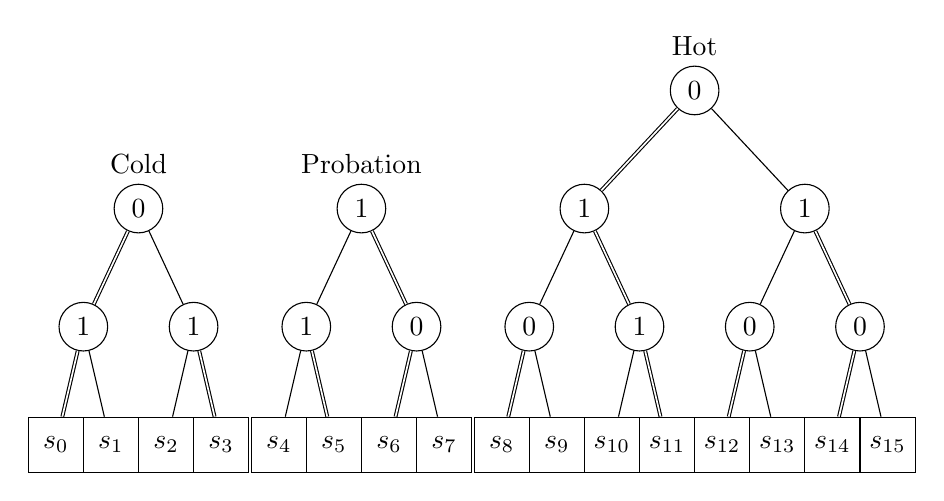
\begin{tikzpicture} [
  every node/.style={draw,distance=12mm},
  level 0/.style={circle},
  level 1/.style={circle,sibling distance=28mm},
  level 2/.style={circle,sibling distance=14mm},
  level 3/.style={rectangle,minimum size=7mm,inner sep=0,sibling distance=7mm}
  ]
  % \node (n0) [circle, label=left:Hot] {0}
		% child [circle, sibling distance=28mm] {
		\node [circle, label=above:Hot] (n2) {0}
      child {
        node (n5) {1}
        child {
          node (n11) {0}
          child {
            node (n23) {$s_8$}
          edge from parent [double]}
          child {
            node (n24) {$s_9$}
          }
        }
        child {
          node (n12) {1}
          child {
            node (n25) {$s_{10}$}
          }
          child {
            node (n26) {$s_{11}$}
          edge from parent [double]}
        edge from parent [double]}
      edge from parent [double]}
      child {
        node (n6) {1}
        child {
          node (n13) {0}
          child {
            node (n27) {$s_{12}$}
          edge from parent [double]}
          child {
            node (n28) {$s_{13}$}
          }
        }
        child {
          node (n14) {0}
          child {
            node (n29) {$s_{14}$}
          edge from parent [double]}
          child {
            node (n30) {$s_{15}$}
          }
        edge from parent [double]}
      };
			\node [
				circle,
				left=22mm of n5,
				label=above:Probation
			] (n4) {1}
				child [circle,sibling distance=14mm] {
          node (n9) {1}
					child [rectangle,minimum size=7mm,inner sep=0,sibling distance=7mm] {
            node (n19) {$s_4$}
          }
					child [rectangle,minimum size=7mm,inner sep=0,sibling distance=7mm]{
            node (n20) {$s_5$}
          edge from parent [double]}
        }
				child [circle,sibling distance=14mm] {
          node (n10) {0}
					child [rectangle,minimum size=7mm,inner sep=0,sibling distance=7mm]{
            node (n21) {$s_6$}
          edge from parent [double]}
					child [rectangle,minimum size=7mm,inner sep=0,sibling distance=7mm]{
            node (n22) {$s_7$}
          }
        edge from parent [double]};
	\node [left=22mm of n4, circle, label=above:Cold](n3) {0}
		child [circle, sibling distance=14mm] {
				node (n7) {1}
				child [rectangle,minimum size=7mm,inner sep=0,sibling distance=7mm] {
					node (n15) {$s_0$}
				edge from parent [double]}
				child [rectangle,minimum size=7mm,inner sep=0,sibling distance=7mm] {
					node (n16) {$s_1$}
				}
			edge from parent [double]}
			child [circle, sibling distance=14mm]{
			node (n8) {1}
			child [rectangle,minimum size=7mm,inner sep=0,sibling distance=7mm]{
				node (n17) {$s_2$}
			}
			child [rectangle,minimum size=7mm,inner sep=0,sibling distance=7mm]{
				node (n18) {$s_3$}
			edge from parent [double]}
		};
\end{tikzpicture}
\end{center}
  \caption{3Tree metadata structure, with separated Cold, Probation, and Hot subtrees}
  \label{fig:3tree}
\end{figure*}


\section{Experiment Methodology}

% Eviction set functions
To evaluate 3Tree in comparison to other algorithms in their defense
against eviction set-based cache priming, % TODO: maybe change this to "eviction set function"
we implement a cache simulator to represent an attacker.
We simulate a single cache set to replicate a single target for an attacker,
and we assume that the attacker has already discovered and minimized an eviction set
of addresses for this cache set.
For a given cache replacement policy and a memory access pattern,
we touch addresses in the cache until the cache is full of attacker-provided memory,
and we record the number of touches required to do this.
As some touching patterns are never able to fill caches with certain replacement
algorithms, we limit the simulator to 100,000 touches and record this as DNF
(did not finish).
Additionally, as most replacement algorithms choose an eviction candidate
based on the cache state, we assume a uniform distribution of possible cache states
and choose one at random.
We conduct 64 trials for each algorithm-pattern pair to account for this randomness.
For each replacement algorithm, we take the touching pattern with the least
required address touches as the experimental difficulty of the algorithm.

Notably, this simulator counts the number of memory accesses required to prime the cache set
but does not include checks an attacker may use during the priming to determine whether
the cache set is fully occupied.
Periodically checking the cache state greatly increases the number of memory accesses required
and strategic checking algorithms are beyond the scope of this research.
Our results provide a confidence interval within which an attacker may reasonably assume
that a cache is filled.
% What's the p of this confidence interval? figure out when data scripts done

% Performance
To evaluate the performance of 3Tree, we implement the algorithm in the
cycle-accurate gem5 CPU simulator on the PARSEC suite of benchmarks \cite{Parsec}
to reflect common modern computing workloads.
Some of these workloads depend on the memory subsystem more than others,
but we take the benchmark suite as generally representative
of cache workloads.
These benchmarks are evaluated on a simulation of a full Linux system,
which includes syscalls and full operating system interaction.
However, the simulator excludes the memory accesses from the boot process
to isolate the cache access counts to the benchmarks themselves.

\section{Results}

\begin{figure*}
	\begin{center}
		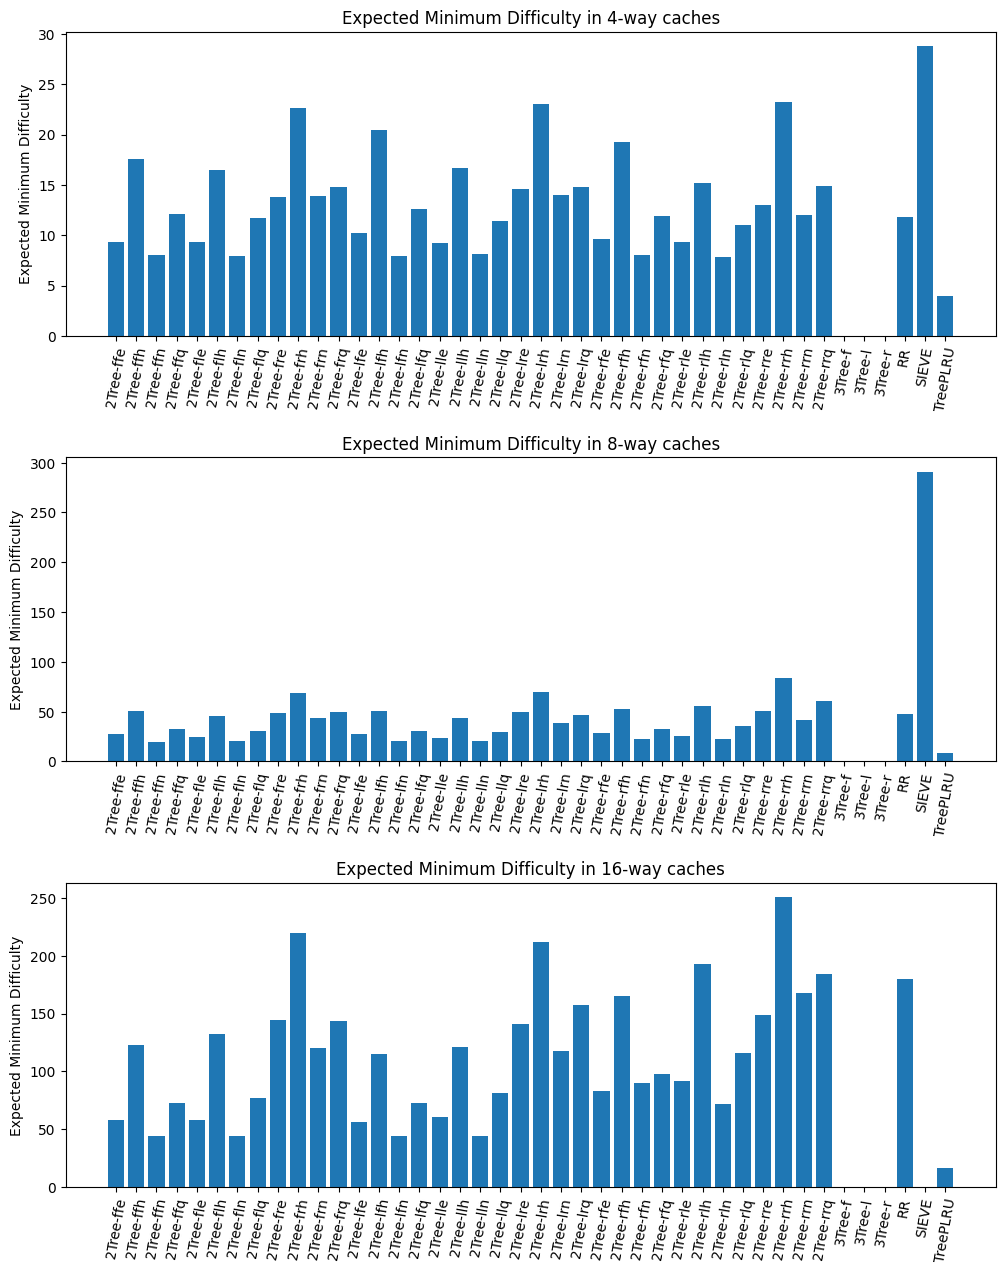
\includegraphics[scale=0.45]{minimum_difficulty}
	\end{center}
  \caption{Expected minimum difficulties of various cache replacement algorithms}
  \label{fig:expected_difficulties}
\end{figure*}

\begin{figure*}
	\begin{center}
		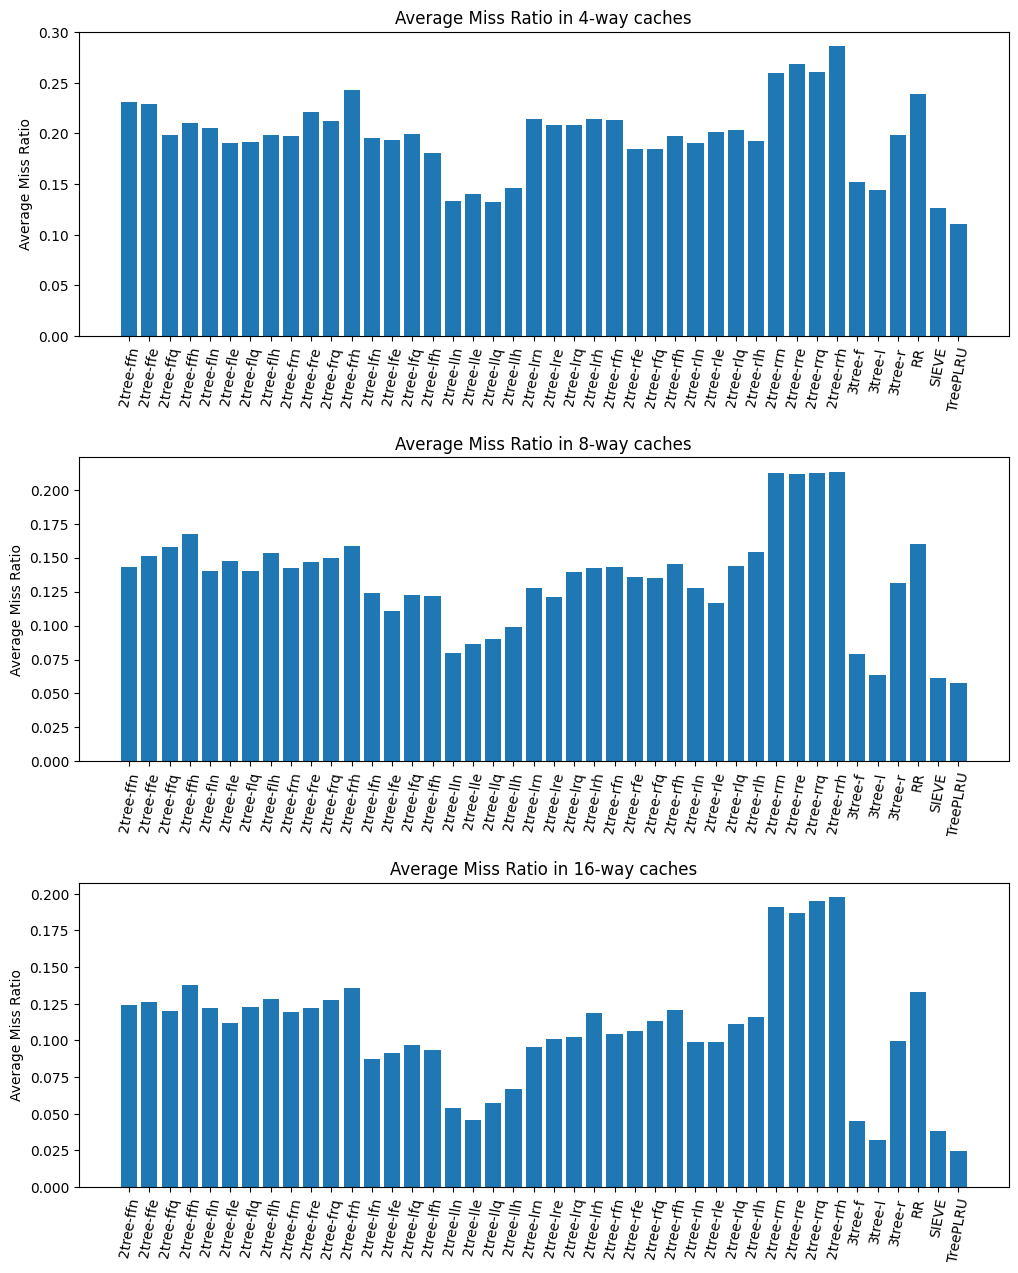
\includegraphics[scale=0.45]{performance}
	\end{center}
  \caption{Average performance of various cache replacement algorithms in PARSEC workloads}
  \label{fig:performance}
\end{figure*}

\subsection{SIEVE Performance}

% Occupation
% Best touch strategy and why
% Comment on low efficacy of SIEVE
% Comment on low efficacy of similar caching strategies

SIEVE performs quite well in both miss ratio and eviction set security.
The experimental expected difficulty is consistently higher than most other cache replacement algorithms,
although it does not match the DNF algorithms and filling a cache set
is only shown to be statistically impossible for a 16-way cache.


Part of its advantage is that it is spatially random.
The selected eviction candidate is dependent on the order of the cache lines;
the specific order of the cache lines and thus the cache state is very difficult to determine
and can change drastically upon any cache operation.
For this reason, SIEVE has a "soft" security advantage against other algorithms,
because an attacker has very little knowledge of whether the cache state is
is in a good or bad position to be primed.
Although specific testing of the probability distribution of 'good' and 'bad' cache states
and thus the expected number of touches an attacker should make to confidently fill the cache
is out of scope for this project,
SIEVE would perform quite well in this regard compared to TreePLRU.

This version of SIEVE does not suffer against Rowhammer attacks, either.
Notably, if new cache objects are added with the visited bit unset, SIEVE would peform exceptionally poorly.
This is because an attacker only needs a target address
$s_t$ and a congruent address $s_c$ to carry out the attack.
First, they touch $s_t$, which finds the first unvisited line and evicts it.
Then, they touch $s_c$, which finds $s_t$ as the new first unvisited line and evicts it.
Then, they repeat these two touches alternatingly, which makes Rowhammer possible
with only twice as many memory accesses as DRAM hits.
Luckily, we do not use this variant of SIEVE in our testing.

Although calculating the exact expected difficulty is not easy,
we include an upper bound for the difficulty.
This is based on the theoretical best touching pattern
on the rare worst possible cache state,
where each of an attacker's accesses evicts their previous access.
This can be handled by touching an address $s_1$,
touching $s_2$ to evict $s_1$ and then touching $s_1$ again to put it back into the cache,
and so on for each of the addresses in the eviction set.
This results in $\frac{a^2}{2}$ accesses to fill the cache set.
Notably, implementing this algorithm is out of scope of this research project.

\begin{equation}
  O(D_g(\text{SIEVE})) = O(D_{Em}(\text{SIEVE})) = a^2
  \label{eq:sieveed}
\end{equation}

% Performance

\subsection{2Tree Performance}

% Occupation
% Best touch strategy and why
% Comment on decent efficacy of 2Tree in full occupation
% Comment on slashed efficacy of 2Tree in actual timing oracle prevention
% Comment on slashed efficacy of split queues

2Tree performs reasonably well against \textit{full} occupation,
because of the choice probability $c$.
This is because even safe elements have a possibility of being evicted through the probation queue.
An attacker may promote an object through extra touches into the hot queue,
but evict their own eviction set addresses with a touch in the probation queue.
Notably, because of the root node that switches between the probation and safe subtrees,
it is equally likely to select an eviction candidate from one of the $a/4$ probation subtree lines
as it is to select an eviction candidate from one of the $a/2$ safe subtree lines.
This means that, upon promotion, objects are likely to be placed in probation
and are at risk of spontaneous eviction.

Calculating the specific expected difficulty is a long combinatorial problem
that can be modeled as a finite state automata.
Calculating these finite states is infeasible by hand,
and modeling them mathematically or in a simulation is out of scope of this research project.

However, 2Tree and other strictly segmented replacement algorithms like TwoQ
suffer in actual performance against timing oracles.
Additionally, 2Tree performs especially poorly against Rowhammer for the same reason.
An attacker may only fill up the cold queue with eviction set addresses
and, depending on the $c$ value of the probation queue, will have a
$1 - c$ chance of a subsequent touch selecting the cold queue as the target location
in the cache.
In this case, a touch of the target address would result in a cache miss and a DRAM hit,
as required by the Rowhammer attack.
For low $c$, it is possible to have a higher cache bypass rate than by filling the whole cache,
as well as a higher rate than simpler algorithms like LRU, given the smaller size of the
cold queue compared to the whole cache set.
Notably, we test the full occupation of the cache in our experimentation,
although real use for timing oracles would result in much lower experimental difficulty values.

Thus, we calculate the guarantee difficulty $D_g$ for 2Tree:

\begin{equation}
	D_g(\text{2Tree}) = \frac{a}{4c} + \frac{a}{4(1-c)}
	\label{eq:2treegd}
\end{equation}

This decreased security holds for any replacement algorithm where new elements can only go
into a subset of the cache lines.
To prime the cache set and form a timing oracle,
an attacker only needs to occupy this subset of the cache with their own newly-placed objects.
To incur cache bypass for Rowhammer, an attacker again only needs to occupy this subset
of the cache to guarantee that their next touch will be a RAM access.

Finally, although this is outside the scope of this work,
it would be simple to implement set dueling with a switch between different $c$ values.
The performance difference between caches with $c=0$ and $c=0.5$ and intermediate values
differs between different benchmarks, as seen in Figure \ref{fig:performance}.
As a hardware implementation, this would not introduce any complexity within the cache set,
instead requiring a global switch affecting the random value generator.
It would not be difficult to implement a similar switch for the replacement algorithms used,
although this introduces more complexity than altering $c$.
FIFO and PLRU only differ in the logic of touching an element already in the cache,
and Random Replacement alters the use of the tree altogether,
meaning a set dueling architecture would have to introduce considerable hardware logic
into each cache set, increasing hardware footprint and energy usage.
Furthermore, this would not be useful for performance.
Across different workloads,
PLRU is consistently shown to be dominant for performance when used in the hot queue,
as shown in figure [cite].
In the cold queue, PLRU is shown to be more performant in some workloads,
and FIFO more dominant in others.
However, the performance difference is minimal:
in workloads where FIFO was better, it was better by an average of 5.1\%,
and in workloads where PLRU was better, it was better by an average of 4.7\%.
With such a small difference, it may be counterproductive to introduce cold queue-specific set dueling
and its subsequent increase in energy and space usage.

\subsection{3Tree Performance}

% Best touch strategy and why
% Comment on fixing problem with fully-segmented 2Tree
% Performance

Out of the proposed algorithms, 3Tree performs the best on average in PARSEC benchmarks.
It performs better than all variants of 2Tree and better than SIEVE by 0.5 percentage points.
However, it is still unable to match the all-round performance of TreePLRU,
and falls 1.7 percentage points behind.
Future work could tune the algorithm and its choice probabilities to determine
a variant more performant than TreePLRU.

3Tree fixes the security issue present in 2Tree and other segmented caches
by allowing new cache objects to be placed in any of the cache lines,
albeit with different probabilities for the probation and hot queues.
Thus, for an attacker priming the cache, all cache lines must be filled to guarantee
that a subsequent access by a victim will be detected with the timing oracle.

Using set dueling on this algorithm can add to the security performance of the algorithm.
The optimal memory access pattern changes is different between the two variants,
which introduces difficulty in the cache priming process \cite{EvictionSetsAtScale}
as there is no trivial way for an attacker to determine the cache replacement algorithm variant.

Additionally, set dueling may greatly increase the miss rate performance of the replacement algorithm.
Dynamically switching between a variant with a big cold queue and one with a big hot queue
allows the cache to react to different workloads.
Processes that access many objects a few times each may better benefit from a big cold queue,
and processes that access a few objects many time benefit from a big hot queue.


% Some analysis on confidence intervals for cache priming and rowhammer
% Especially for priming: confidence of validity of leaked data

\section{Discussion}

This defense is not meant to work alone.
3Tree cannot completely prevent transient execution attacks or Rowhammer,
nor can any alteration of cache replacement policies
without severely impacting the performance of innocuous processes.
Instead, increasing the difficulty of a cache replacement algorithm
and "making it harder" to complete these attacks
is only meant to make these eviction set-based attacks take longer.
Then, a full attack sequence that relies on eviction sets and often uses them
thousands of time in series \cite{Gofetch} should take considerably longer
and the rate of information leakage should be lower according to the
inverse of the increased difficulty value.

Rowhammer is unique in this regard, as the electromagnetic interference effect
it relies on to flip memory bits depend on very fast repeated DRAM access.
The exact speed of these accesses required to flip bits is inconsistent between
different RAM architectures,
but in all architectures there is a certain access frequency threshold
which the attack requires.
Then, reducing the frequency of cache bypass and DRAM access may reduce the access frequency
below the threshold.
Testing of this effect on actual hardware was out of scope of this research project,
given the need to test many different DRAM architectures.
Additionally, there is room for other similar algorithms and advancements.
For example, modern rowhammer defenses may raise the access frequency threshold
using better electromagnetic isolation techniques,
or another DRAM access reduction technique may better isolate memory accesses to the cache.
In either case, this defense may work well with others
to ensure the maximum expected access frequency is below the frequency required for the attack.

This defense also suffers from adoptibility in real computing systems.
As a hardware defense, it is impossible to inject into existing insecure systems
without completely replacing CPUs with new ones, which is often untenable.
Software defenses are often more powerful and feasible in this regard,
as they can be downloaded in a software update while providing similar security guarantees.
However, cache replacement policies like these are specifically usitable to on-the-fly editing.
2Tree and 3Tree are both based on tree structures with some nodes removed,
so it would be possible to dynamically change the behaviour of each tree node
on insertion and eviction according to these algorithms or other tree-based variants.
This can be used to switch between FIFO, LRU, and Random replacement policies
in each of the subtrees of 2Tree and 3Tree according to the workload presented.
However, the feasibility of these options is questionable,
as caches are made to be as fast as possible,
and the introduction of additional per-set hardware
could greatly increase the latency of the replacement algorithm
and the power draw of the cache set circuit.
However, other than in new CPUs, this defense excels in protecting old, large software systems
that cannot be updated.
In this case, the hardware may be the only component that can be updated for security,
and altering CPUs and their replacement policies around the software they run
may be the only option.

The lack of a specific target for this defense is both a strength and a weakness.
Many other defenses have been created around specific attacks,
including mitigations for Spectre, Meltdown, and Spectre v2.
These defenses are often specifically suited to the attacks they target,
and struggle to defend against other attacks that are made to circumvent them.
By contrast, this defense attempts to defend against the whole class of
eviction set-based attacks instead of a specific one,
and thus proactively affects attacks beyond the currently existing ones.
The Prime+Probe, Evict+Time, and Evict+Reload attack foundations
are the basis of many current attacks and will be used for many attacks in the future.
Decreasing the strength of these attack fundamentals impacts
future cyberattacks in a way that targeted defenses cannot.

Finally, the introduction of extra hardware into the very commonly-used cache circuit
arises questions of the performance characteristics of CPUs that use this.
Although we cannot make specific claims on the performance without energy-measuring models
and more robust latency measurements,
we analyze performance claims in comparison with existing architectures.
In both 2Tree and 3Tree, the use of set dueling to choose between different subtree replacement algorithms
is simple and requires little hardware cost, given that the tree structure is maintained
among the different variants.
Existing Intel processors often use set dueling between the TreePLRU and QLRU algorithms
\cite{EvictionSetsAtScale}, despite the two algorithms being very different from one another.
TreePLRU uses a tree structure very similar to 2Tree and 3Tree,
but QLRU uses per-line metadata similar to SIEVE,
along with very similar sequential logic likely also based on a priority encoder.
Because this is viable in commercial CPUs, we deem our use of set dueling for subtree algorithms
as an insignificant factor in performance.

However, our implementations of 2Tree and 3Tree suffer compared to TreePLRU
because they swap cache objects between different lines to move data to a more or less safe subtree.
This requires a 64 byte bus connected to each of the 64 byte cache lines
to allow them to transport data to a hub which should connect each of the busses to each of the others.
Compared to the rest of the circuit requirements of these algorithms,
this is not an insignificant added complexity, and may add to the power draw of the cache.

Despite the performance concerns,
replacement algorithm latency is still not a large factor in the performance of the CPU.
Modern compiler techniques such as prefetching can heavily diminish the importance
of a performant replacement algorithm.
They may request data in memory long before it is used to ensure it is in the cache when it is needed,
which reduces the cost of a cache miss
and may completely remove the cost of a replacement algorithm circuit with a longer critical path.
Prefetching may additionally have implications in the security against both Rowhammer
and other eviction set attacks,
but study of these effects is beyond the scope of this study.
Additionally, most modern CPUs fetch the data from the cache before updating the replacement policy metadata
according to the touch.
This completely removes the cost of a replacement algorithm's longer critical path
for single memory accesses
and may still reduce the latency for repeated accesses of the same data,
depending on the speed of these accesses.

2Tree is relatively bad in performance and exhibits exceptionally bad security characteristics.
Meanwhile, 3Tree and SIEVE are both viable algorithms for a balance of security and performance.
They greatly increase a CPU's defense against eviction set attacks,
and with proper tuning and optimization may be more performant than state-of-the-art replacement policies.

% performance implications
  % prefetching, etc. to diminish the importance of cache misses
  % photonics and in-memory compute as an additional solution, bypassing cache requirement

% PARSEC

%-------------------------------------------------------------------------------
\bibliographystyle{acm}
\bibliography{sources}

%%%%%%%%%%%%%%%%%%%%%%%%%%%%%%%%%%%%%%%%%%%%%%%%%%%%%%%%%%%%%%%%%%%%%%%%%%%%%%%%
\end{document}
%%%%%%%%%%%%%%%%%%%%%%%%%%%%%%%%%%%%%%%%%%%%%%%%%%%%%%%%%%%%%%%%%%%%%%%%%%%%%%%%

%%  LocalWords:  endnotes includegraphics fread ptr nobj noindent
%%  LocalWords:  pdflatex acks
